\subsection{Initial Exploration}

Before diving into the analysis, we started by taking a look at the structure of the dataset. It contains private messages exchanged on an online social network at UC Irvine. Each row represents a message with three main pieces of information:

\begin{itemize}\setlength{\itemsep}{0pt}
    \item \texttt{SRC}: the ID of the sender
    \item \texttt{TGT}: the ID of the receiver
    \item \texttt{UNIXTS}: the timestamp of the message in Unix time format
\end{itemize}

Since Unix time isn't very human-readable, we converted the timestamps into proper datetime objects. We also adjusted them to Pacific Time (America/Los\_Angeles), which is the timezone used at UC Irvine. This made it easier to interpret the data accurately.

As a first step, we asked ourselves a few basic questions: \textit{"How big is this dataset? How many users are involved? Over what time period were these messages exchanged?"}

\begin{itemize}\setlength{\itemsep}{0pt}
    \item Number of messages: 59,835
    \item Unique users: 1,899
    \item Time span: April 15, 2004 to October 26, 2004
\end{itemize}

These numbers show that the dataset covers just over six months of messaging among nearly 2,000 users.

\subsection{Message Volume Over Time}

To get an idea of how activity changed over time, we counted how many messages were sent each day. As shown in Figure~\ref{fig:messages-per-day}, there are clear fluctuations, with some noticeable spikes. These might match up with academic deadlines or social events on campus.

\begin{figure}[H]
    \centering
    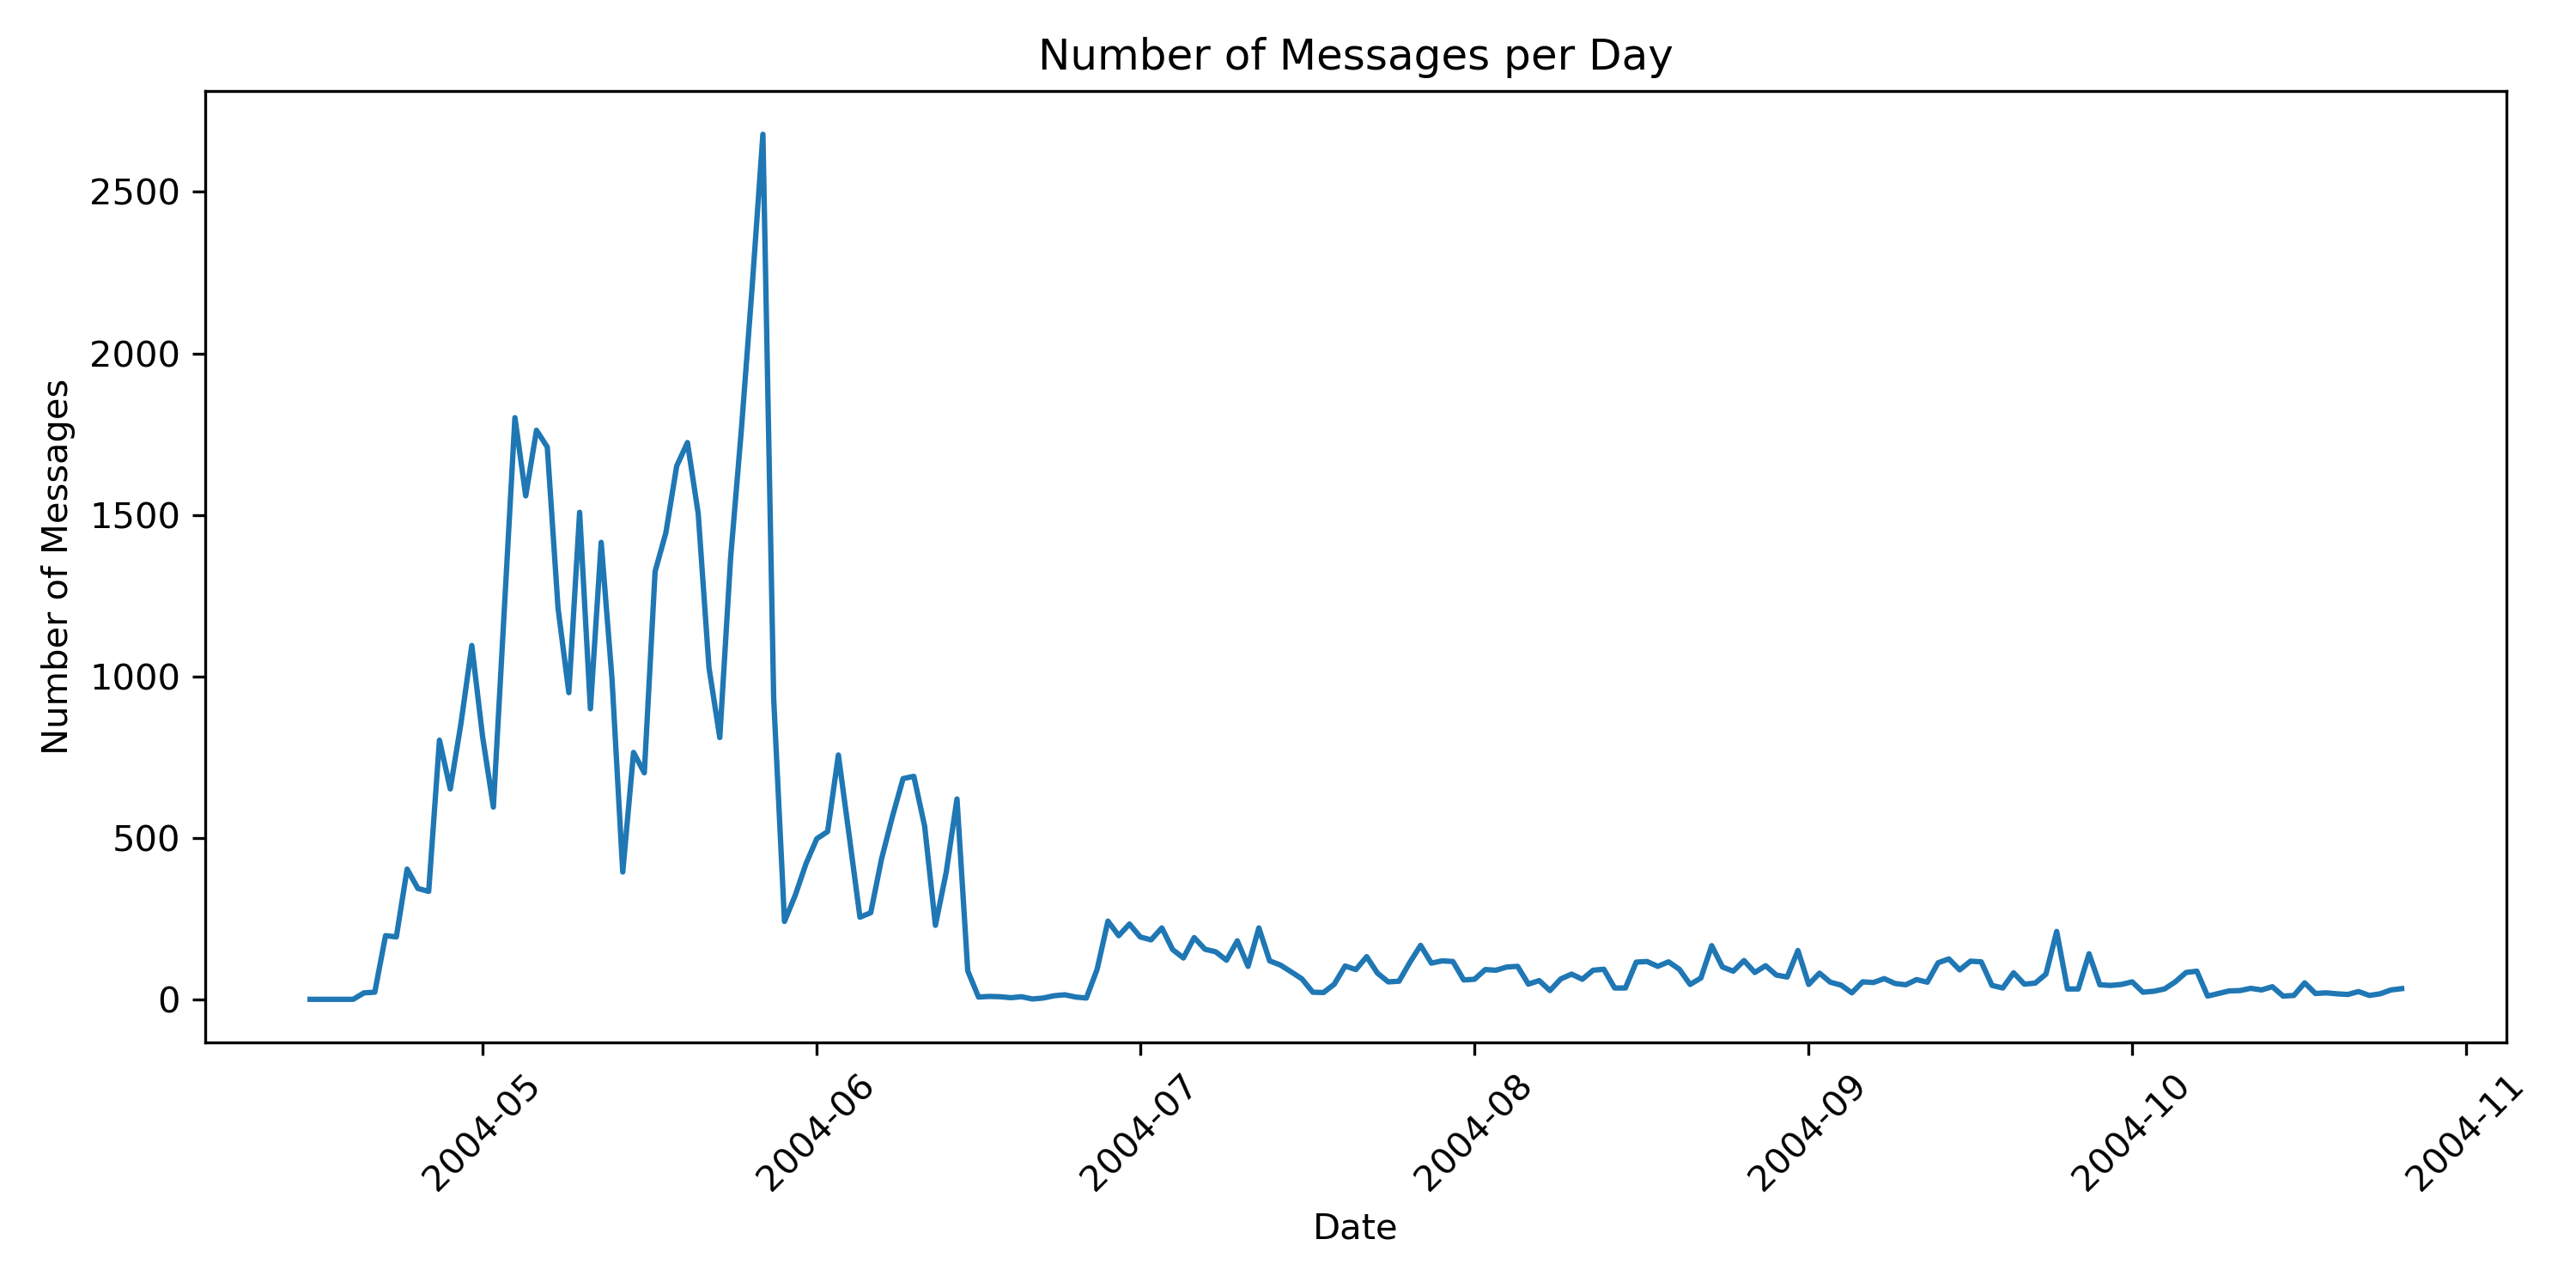
\includegraphics[width=0.5\linewidth]{../Images/messages_per_day.png}
    \caption{Daily message volume over time}
    \label{fig:messages-per-day}
\end{figure}

One thing worth pointing out is that the busiest period falls between April and June 2004, which lines up with UC Irvine's spring term. This supports the idea that the platform was most used during the academic semester.

\subsection{Temporal Analysis}

Next, we wanted to see if students followed any specific patterns when sending messages. We looked at three time-based breakdowns: by hour of the day, by weekday, and by month. The results are shown in Figure~\ref{fig:temporal-analysis}.

\begin{figure}[H]
    \centering
    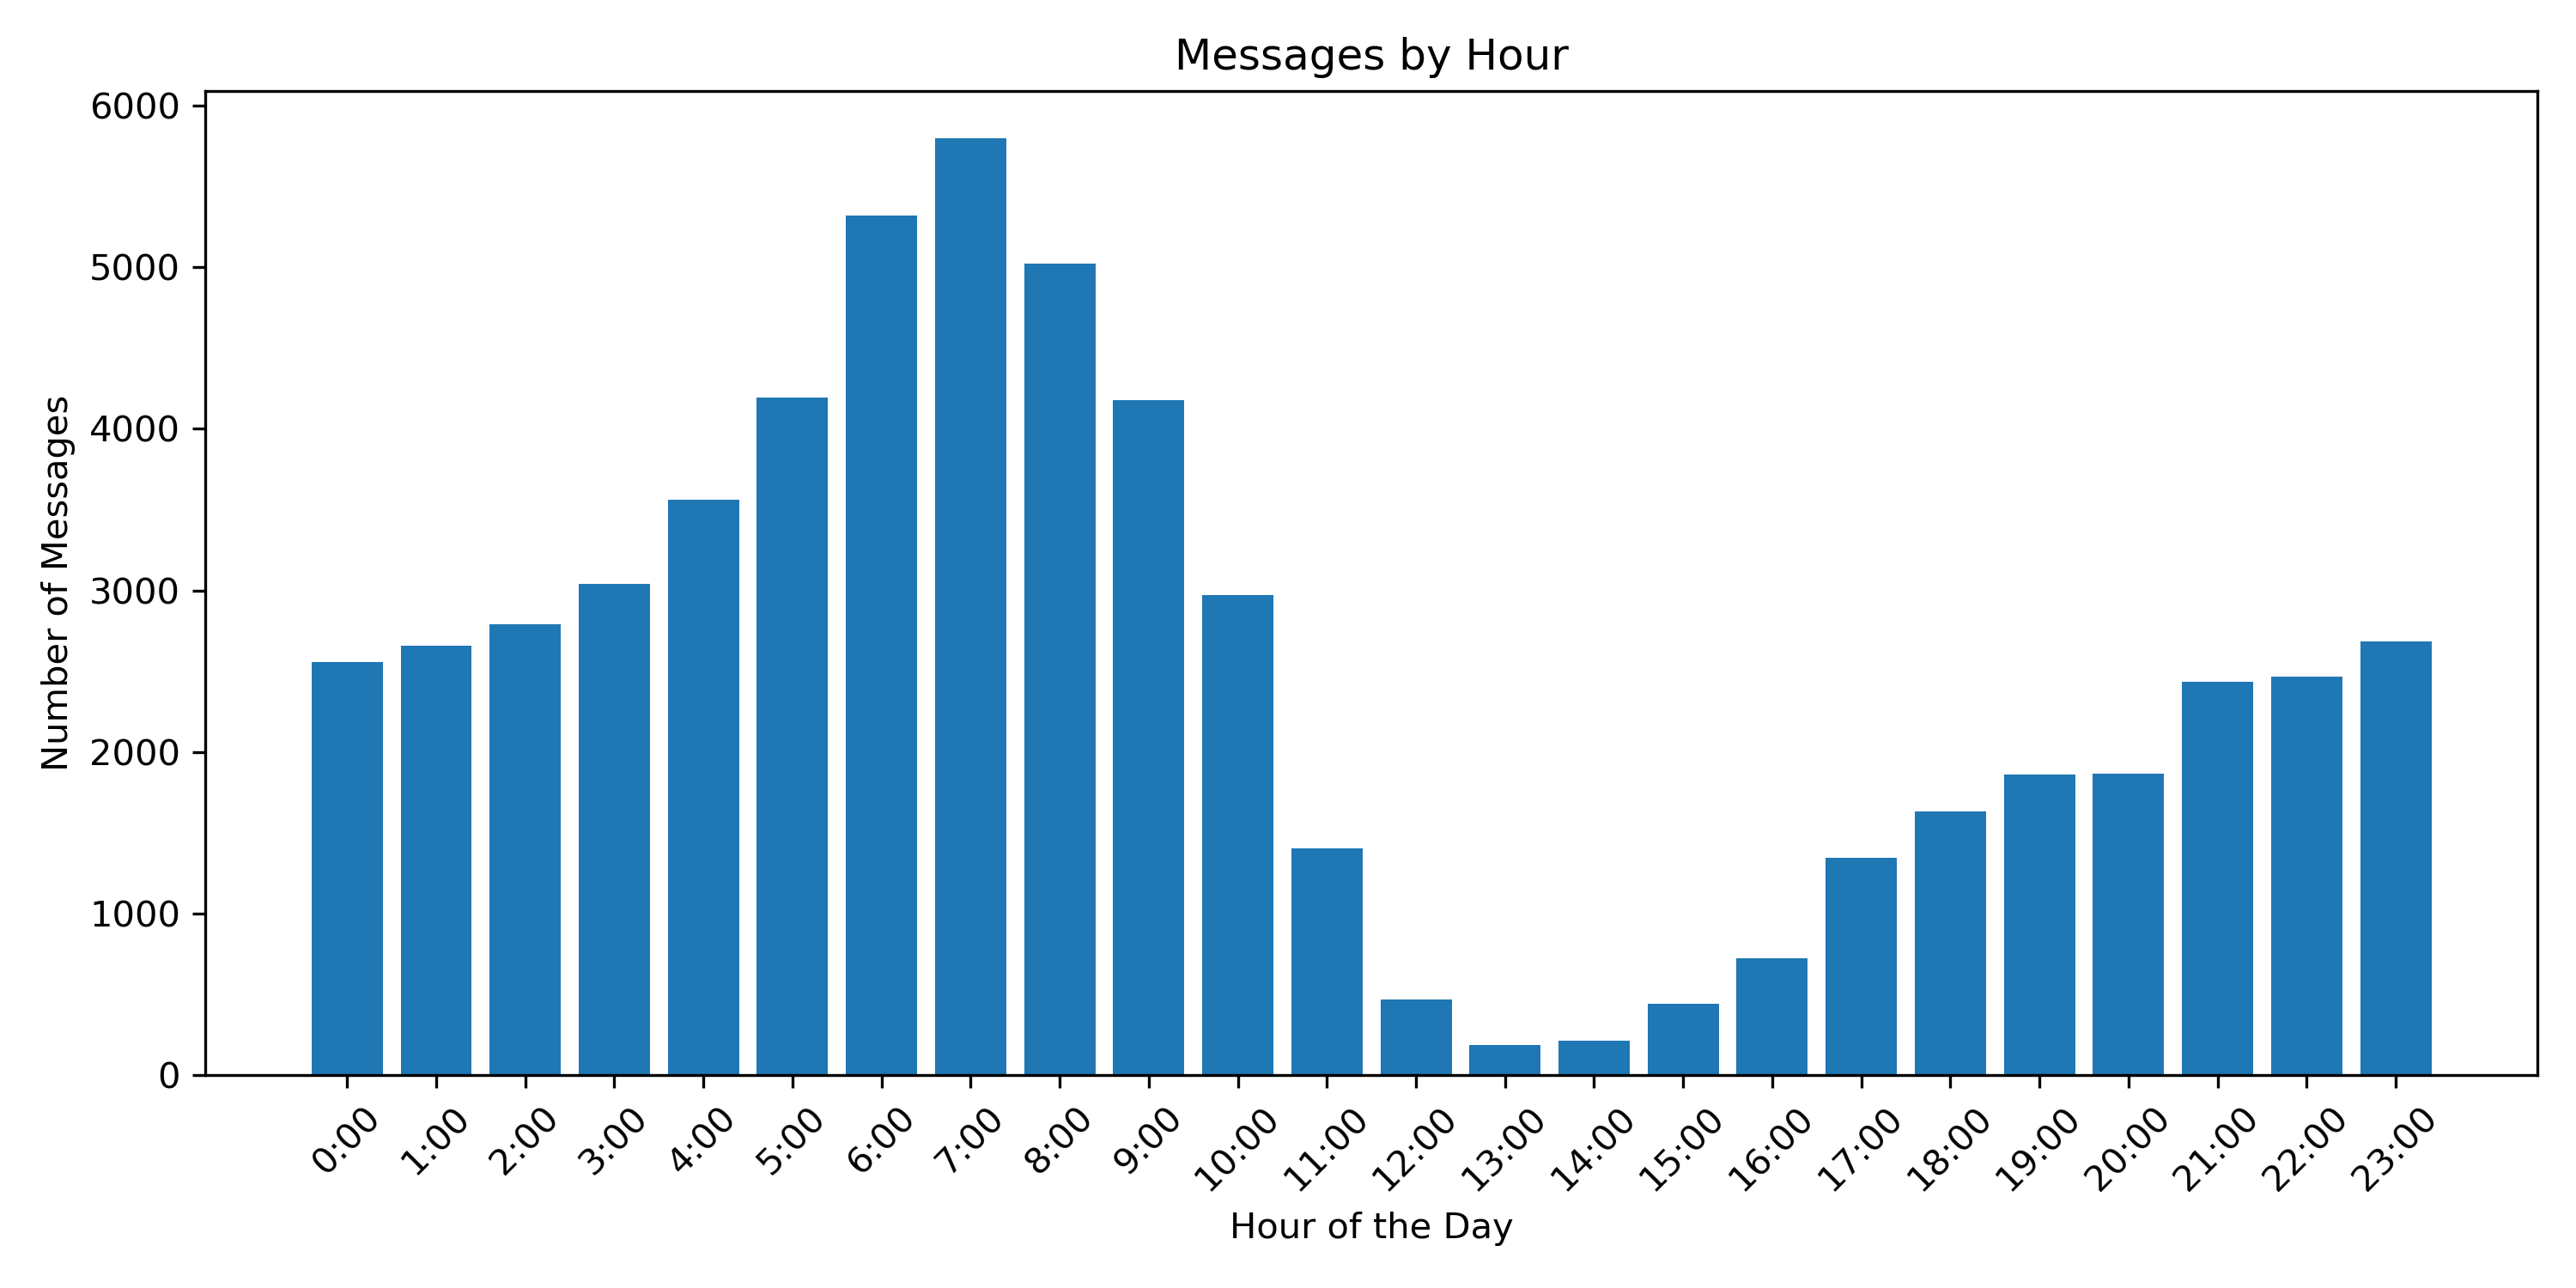
\includegraphics[width=0.3\linewidth]{../Images/messages_by_hourWrong.png}
    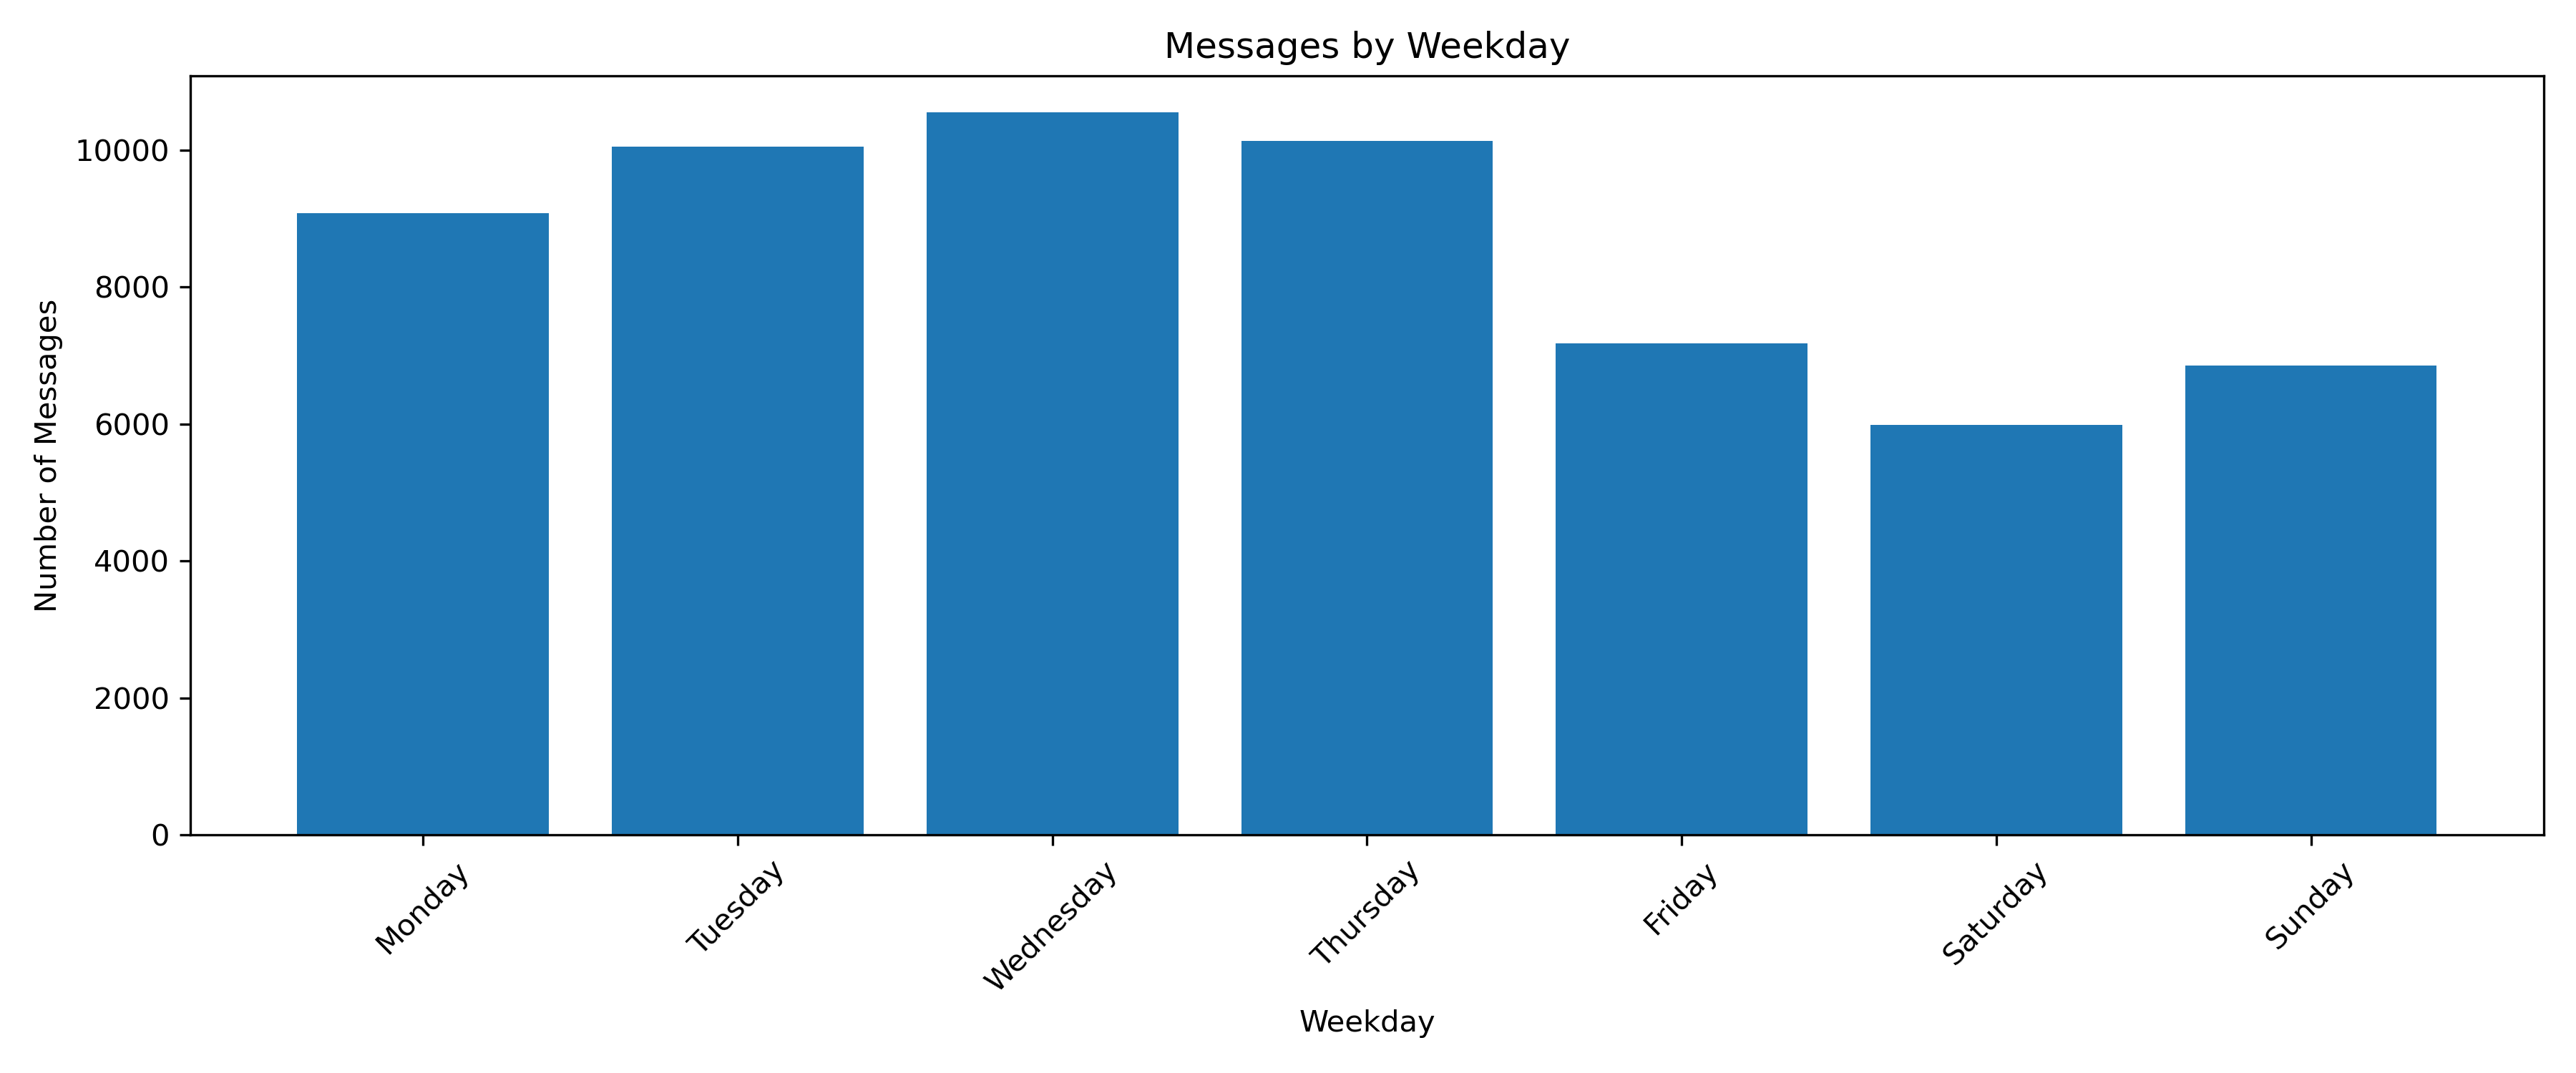
\includegraphics[width=0.3\linewidth]{../Images/messages_by_weekday.png}
    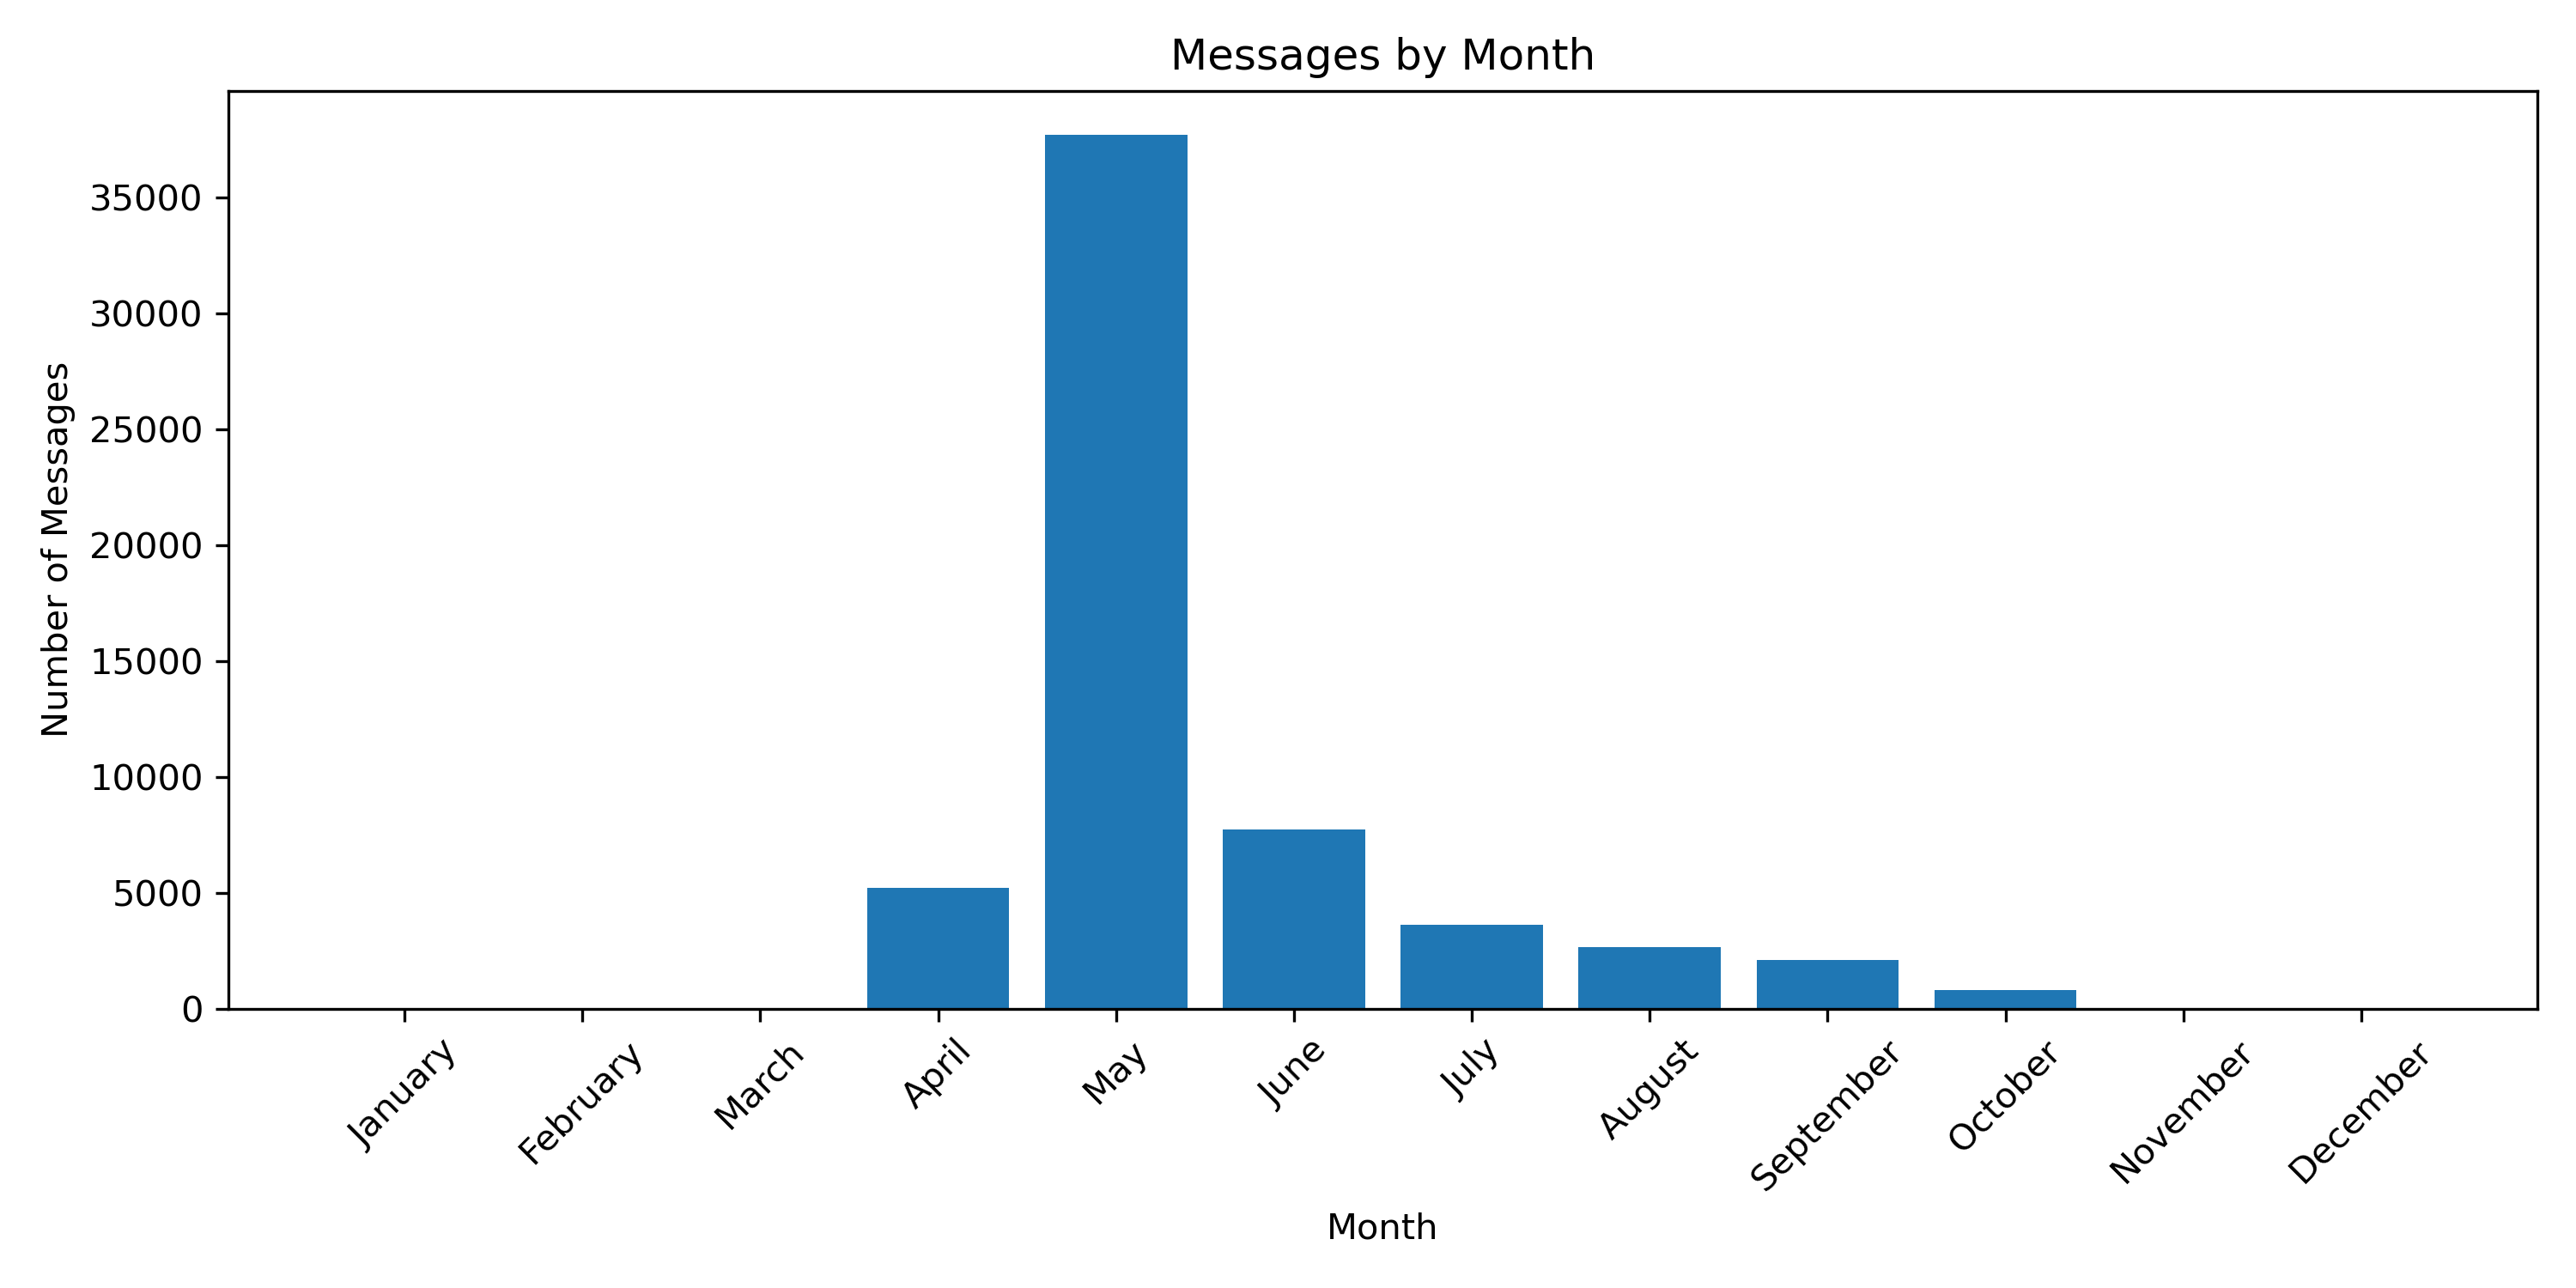
\includegraphics[width=0.3\linewidth]{../Images/messages_by_month.png}
    \caption{Temporal breakdown of message activity by hour, weekday, and month (adjusted to local time)}
    \label{fig:temporal-analysis}
\end{figure}

However, something strange popped up right away: a lot of messages were sent between 5:00 and 8:00 a.m. UTC. That didn't seem right—why would students be so active that early in the morning? That made us think there might be an issue with the timezone.

\subsection{UTC Time Conversion}

Since the dataset is from UC Irvine, which is in the Pacific Time Zone (UTC--7), and the timestamps were in UTC, we figured we needed to adjust the time accordingly. After converting to Pacific Time, the peak shifted to around 10 a.m. to 1 p.m., which made a lot more sense.

\begin{figure}[H]
    \centering
    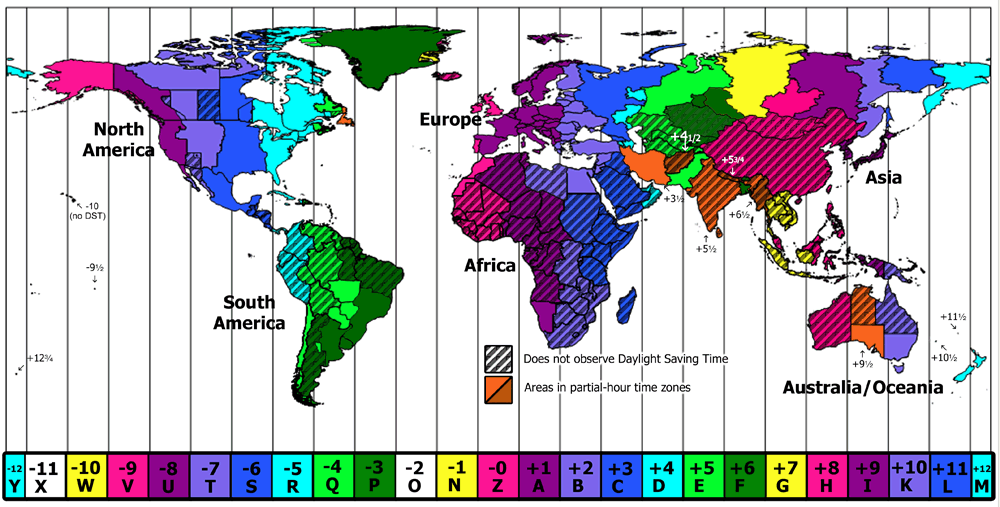
\includegraphics[width=0.3\linewidth]{../Images/UTCmap.png}
    \hspace{10pt}
    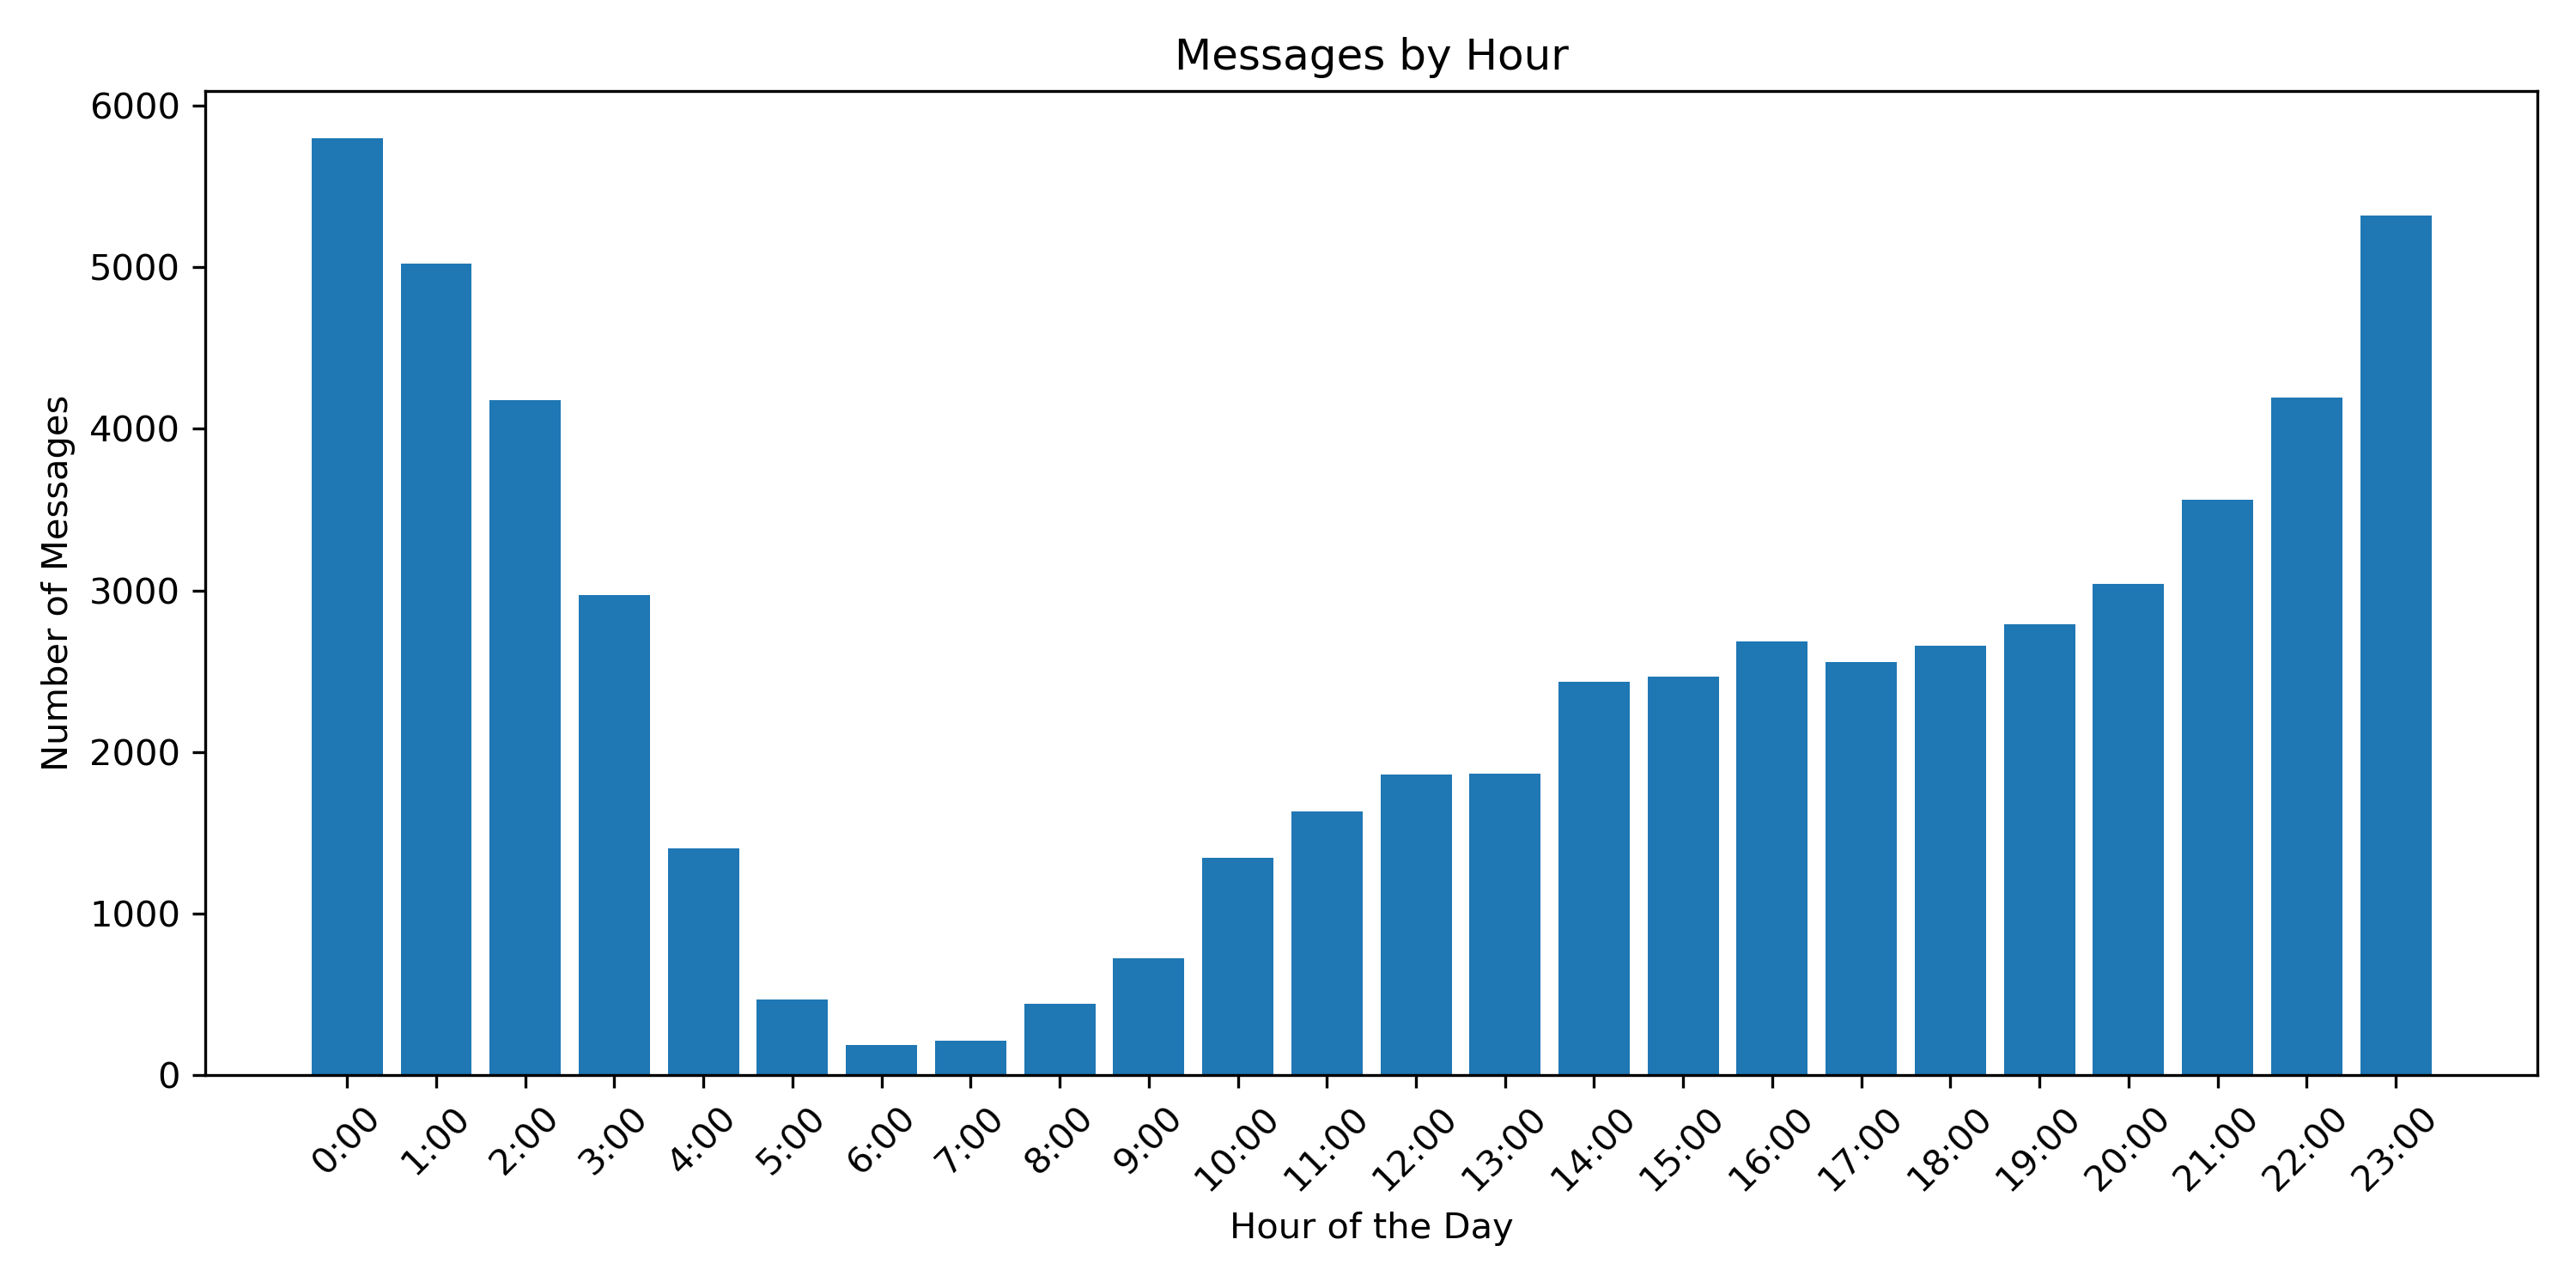
\includegraphics[width=0.35\linewidth]{../Images/messages_by_hour.png}
    \caption{\textbf{Left}: UTC time zone map. \textbf{Right}: Hourly message distribution after conversion to local time}
    \label{fig:hourly-after-conversion}
\end{figure}

This small fix cleared up the confusion. The data was fine—it just needed the correct timezone. With this adjustment, the messaging behavior matched what you'd expect from a student population.

\subsection{Top Users vs Least Users Analysis}

While exploring the data, we noticed that User 234 was particularly active. This got us thinking:

\textit{"Do the most central users behave differently from users who are active but not very well connected in the network?"}

To find out, we used the PageRank algorithm to rank all users and then selected:

\begin{itemize}
    \item The top 10 users by PageRank
    \item The bottom 10 users by PageRank among those with non-zero out-degree (so, users who actually sent messages)
\end{itemize}

We then compared how these two groups behave throughout the day by averaging their message activity hour-by-hour.

\begin{figure}[H]
    \centering
    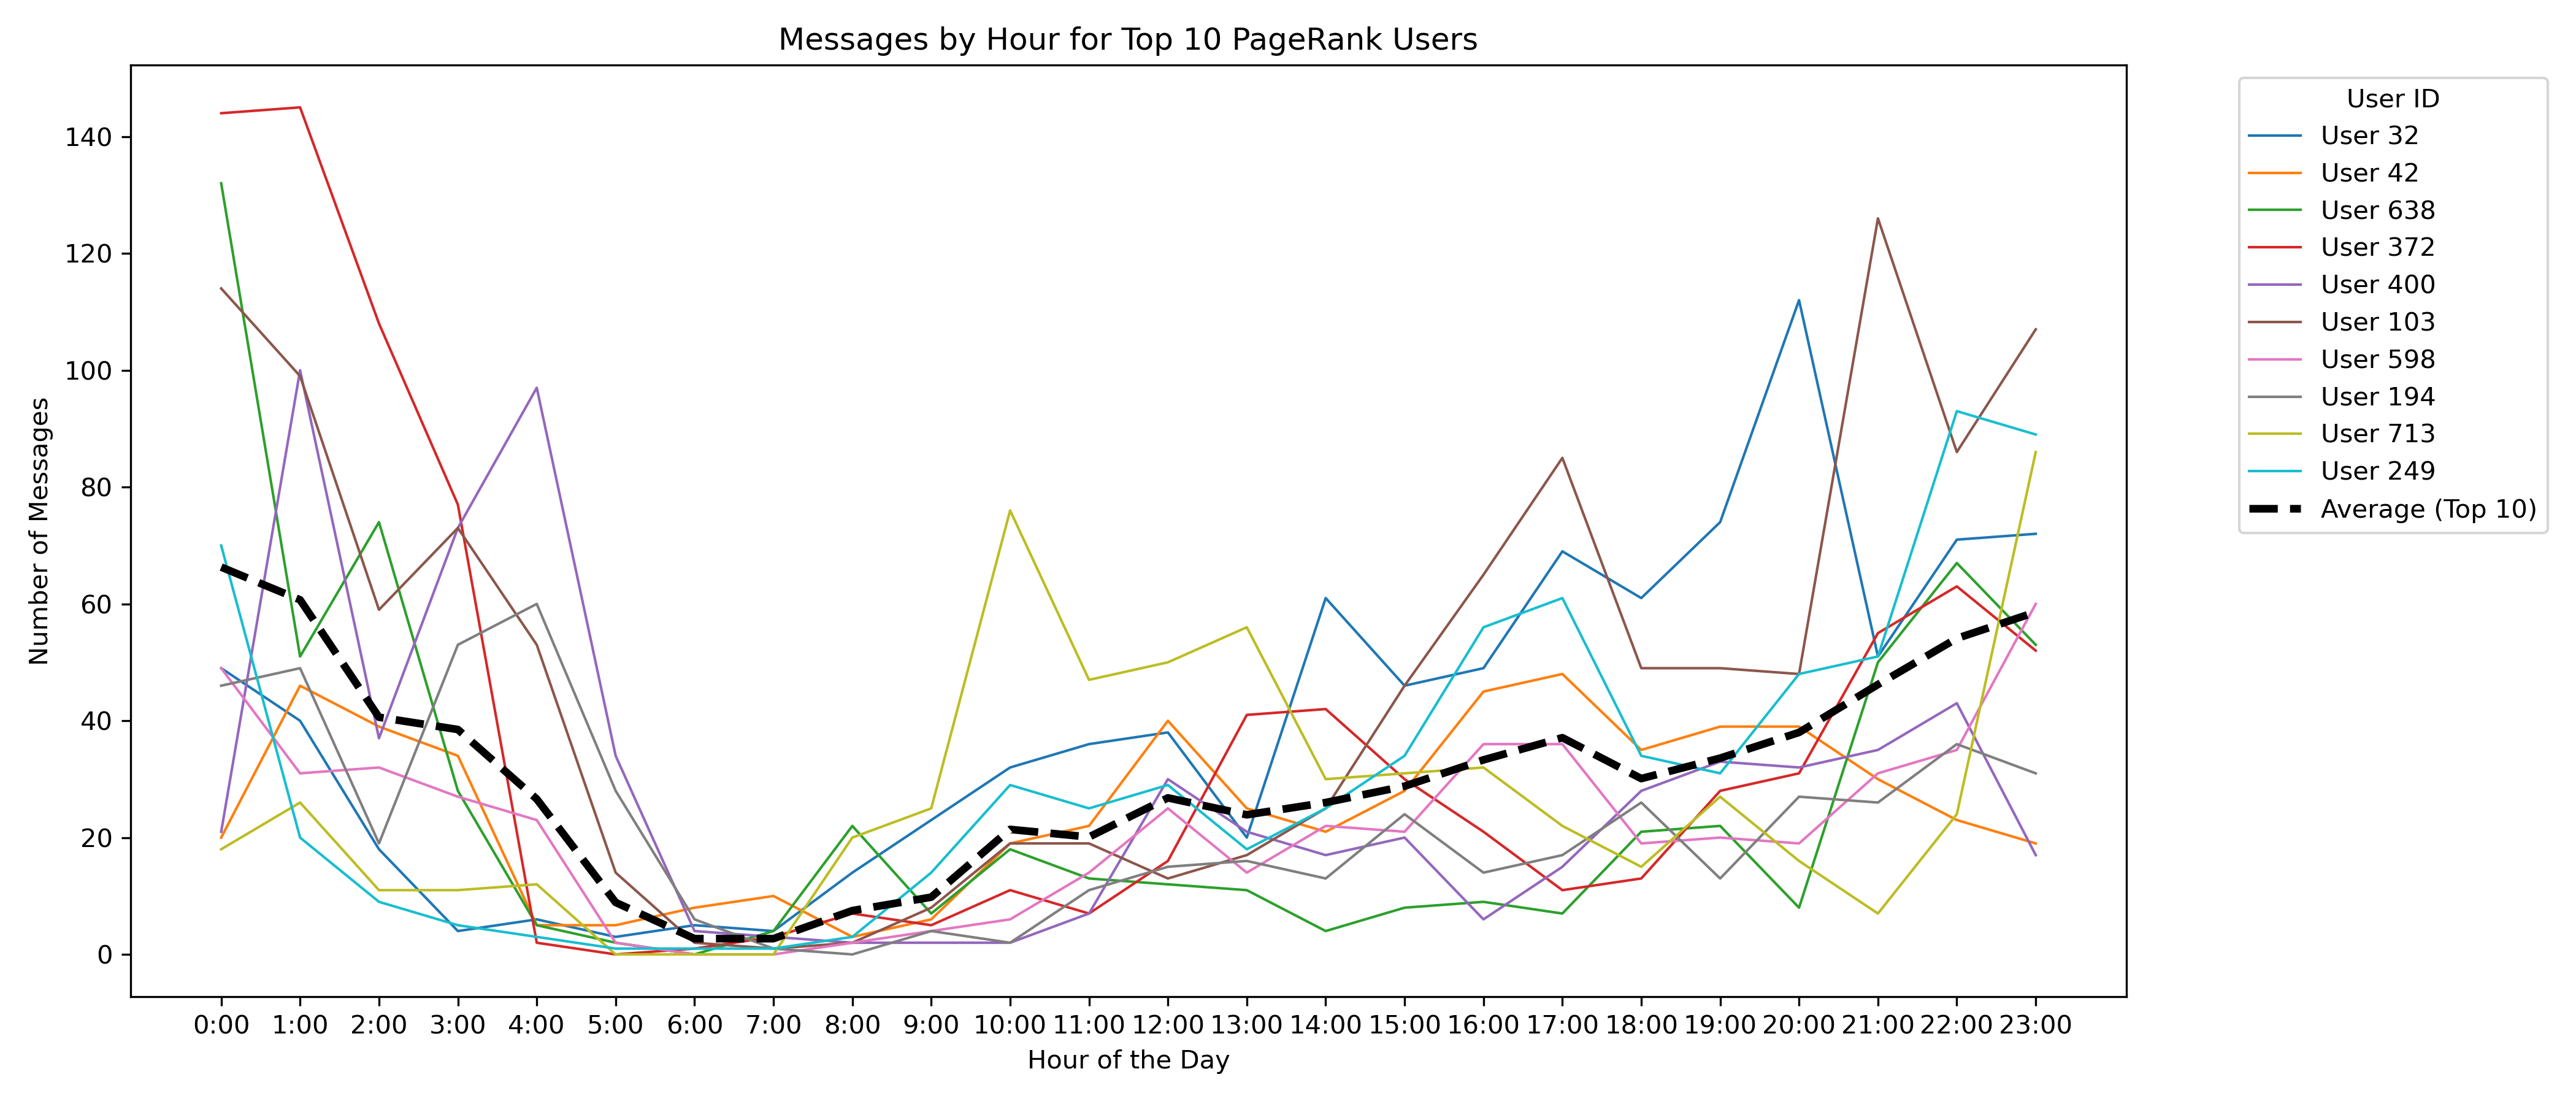
\includegraphics[width=0.45\linewidth]{../Images/top10_users_individual_lines_with_average.png}
    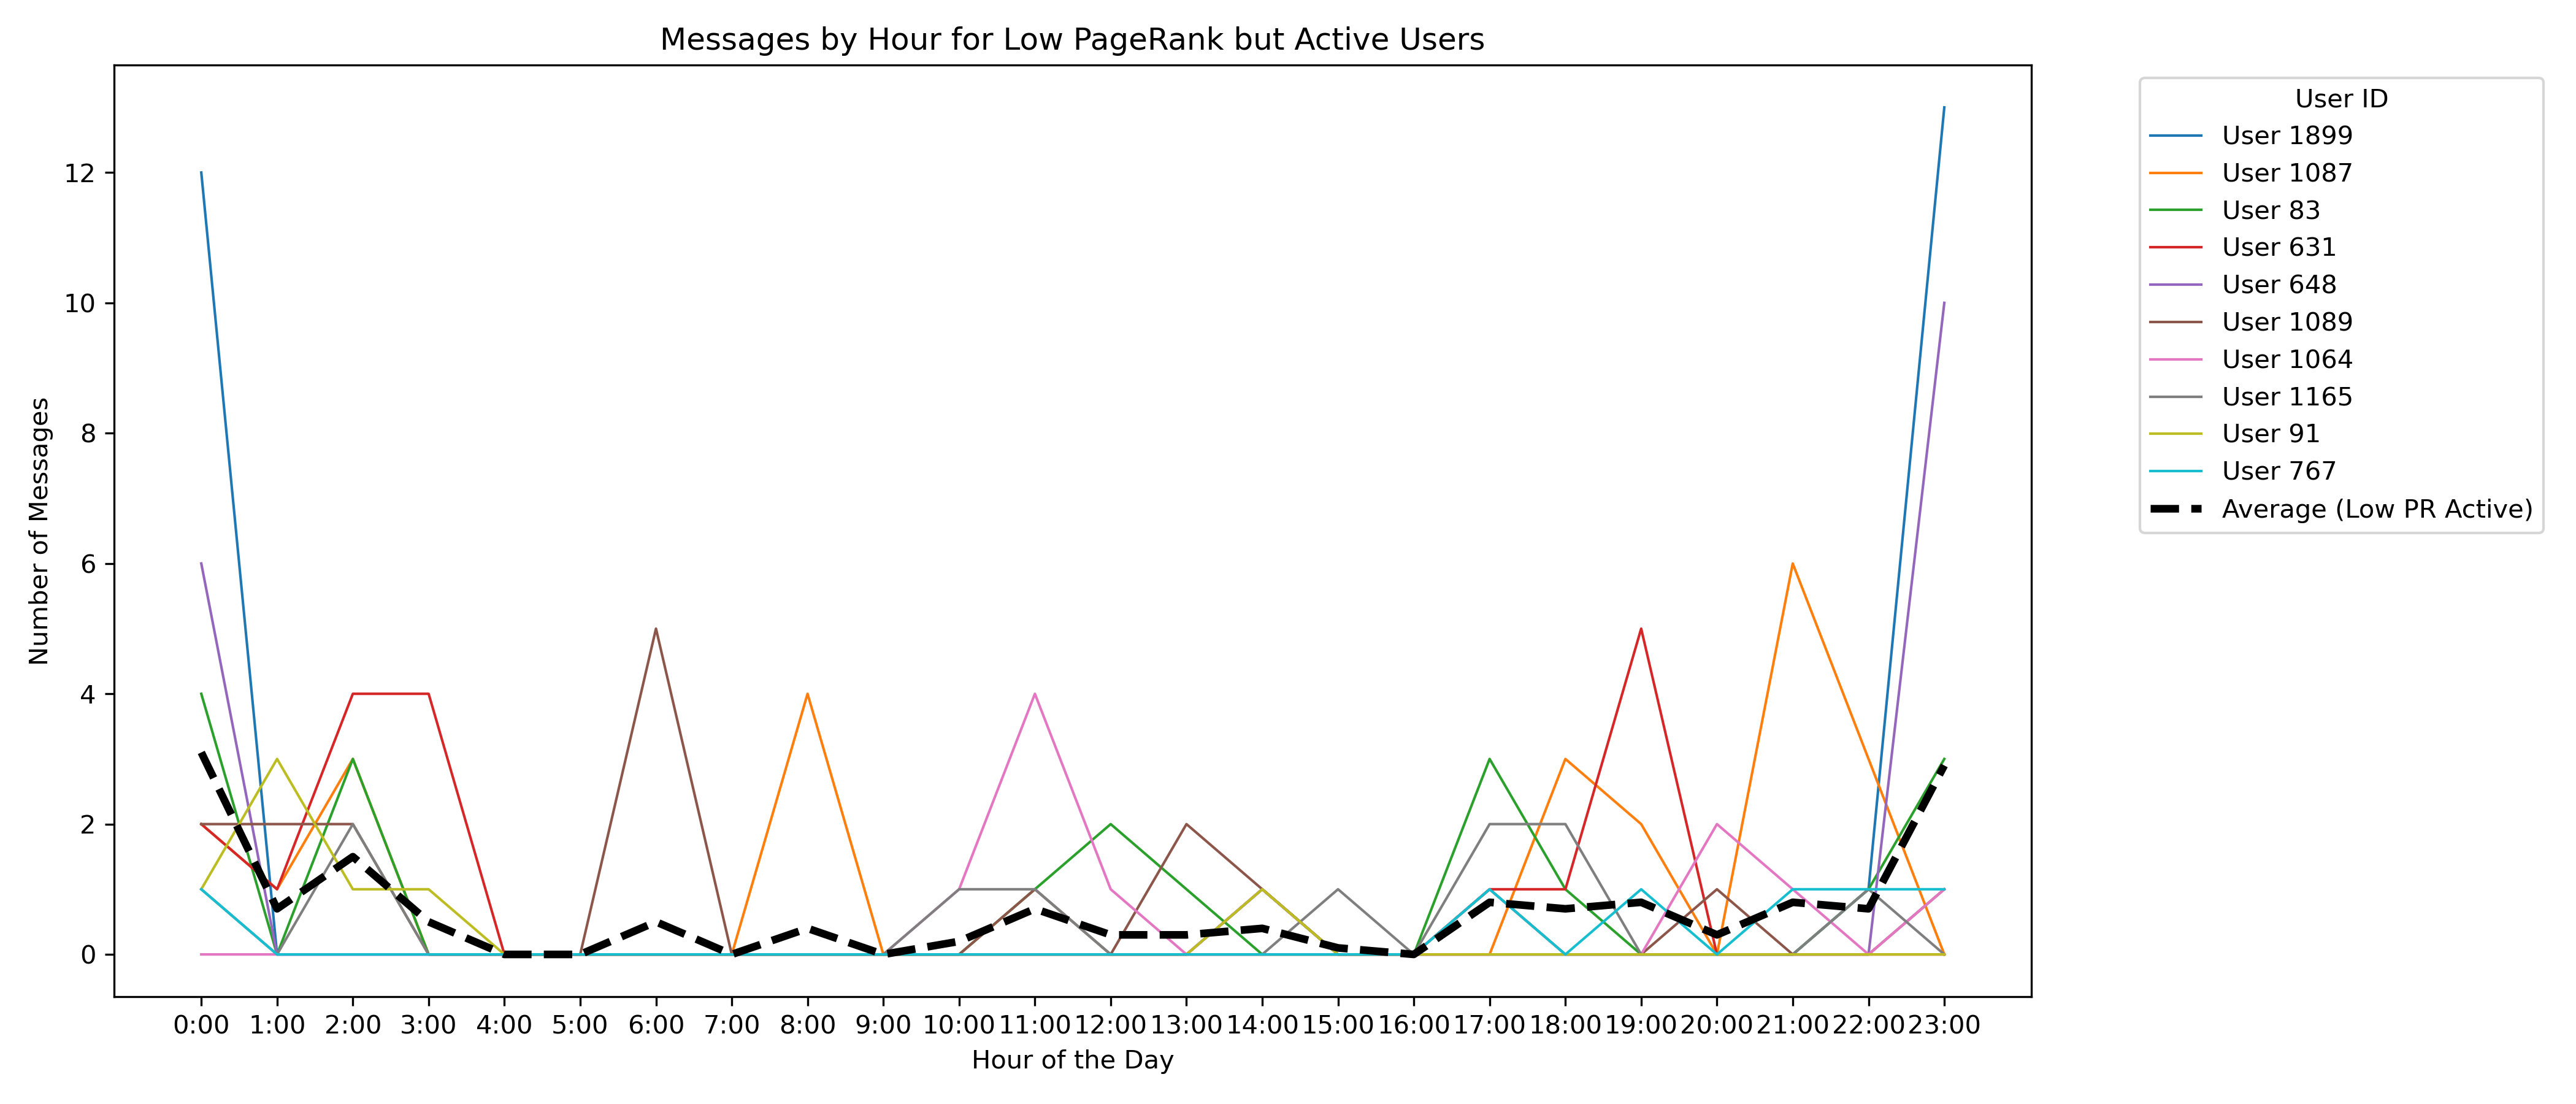
\includegraphics[width=0.45\linewidth]{../Images/low_pr_active_users_with_average.png}
    \caption{Comparison of average hourly activity between top 10 and bottom 10 active PageRank users}
    \label{fig:top-vs-bottom}
\end{figure}

Looking at Figure~\ref{fig:top-vs-bottom}, it seems like the top users have a more stable and consistent messaging pattern throughout the day. Their activity spans many hours with smaller fluctuations. On the other hand, the less central users show a more sporadic and concentrated behavior, often limited to specific times. This could mean that more central users are generally more engaged in ongoing conversations, while less connected users tend to message in bursts.